\subsection{Bereitstellung}
Die einzelnen Komponenten von Elastifeed arbeiten überwiegend autark und ohne einen gespeicherten Zustand.
Dieses Verhalten ermöglicht es uns, einzelne Komponenten individuell zu Skalieren, um etwa die Performance zu verbessern.
Für eine einfache Skalierung kommt eine Container-basierte Architektur zum Einsatz.
Weitere Details zur Implementierung finden sich im Abschnitt "Elastifeed in Kubernetes".

\subsubsection{Linux Container}
Ein Linux Container besteht aus Prozessen, die über eine Kernel-Schnittstelle vom Rest des Systems abgeschottet sind. Ausgeliefert werden Container als ein lauffähiges Image, in dem alle notwendigen Abhängigkeiten für eine Anwendung bereits integriert sind.
Alle Komponenten von Elastifeed sind als Container bereitgestellt.

\subsubsection{Dockerfile}
Um einzelne Komponenten in einem Container bereitzustellen, wird ein \texttt{Dockerfile} genutzt.
In diesem ist ein Basis Image definiert und alle notwendigen Befehle um die Anwendung zu kompilieren.
Bei einem in Golang implementierten Services gestaltet sich dies besonders einfach, da die Anwendung statisch kompiliert wird und in keiner Abhängigkeit zu Systembibliotheken steht.
Einer dieser Services ist in unserer Projektarbeit das Push-Gateway zu Elasticsearch.
Im ersten Schritt wird die Anwendung kompiliert - als Basis-Image dient hierbei das \texttt{golang} Image \cite{god}.

\begin{minted}{docker}

FROM golang:1.12-alpine AS builder

\end{minted}

Anschließend werden notwendige Abhängigkeiten installiert und die Anwendung kompiliert.

\begin{minted}{docker}
RUN apk update && apk add --no-cache git
ENV GO111MODULE=on

WORKDIR $GOPATH/src/github.com/elastifeed/es-pusher

# Copy source files
COPY . .

# Fetch deps dependencies
RUN go get -d -v ./...

# Build and Install executables
RUN CGO_ENABLED=0 GOOS=linux go build ./cmd/entrypoint.go && mkdir -p /go/bin/ && mv entrypoint /go/bin/es-pusher
\end{minted}

Abschließend wird nach dem erfolgreichen Übersetzungsprozess ein minimales Container Image erstellt, welches nur aus der Anwendung besteht.

\begin{minted}{docker}
FROM scratch

COPY --from=builder /go/bin/es-pusher /go/bin/es-pusher

ENV API_BIND=":9090"

ENTRYPOINT ["/go/bin/es-pusher", "-logtostderr=true"]

EXPOSE 9090
\end{minted}

Um Container nicht nach jeder Änderung manuell zu Aktualisieren, verwenden wir die Container-Registry quay.io, die im Zusammenspiel mit Github eine Continuous Delivery Plattform bietet und nach Einchecken einer neuen Version in Github das Container-Image automatisiert neu erstellt. \autoref{deployment:image:quay}

\begin{figure}[t]
  \centering
  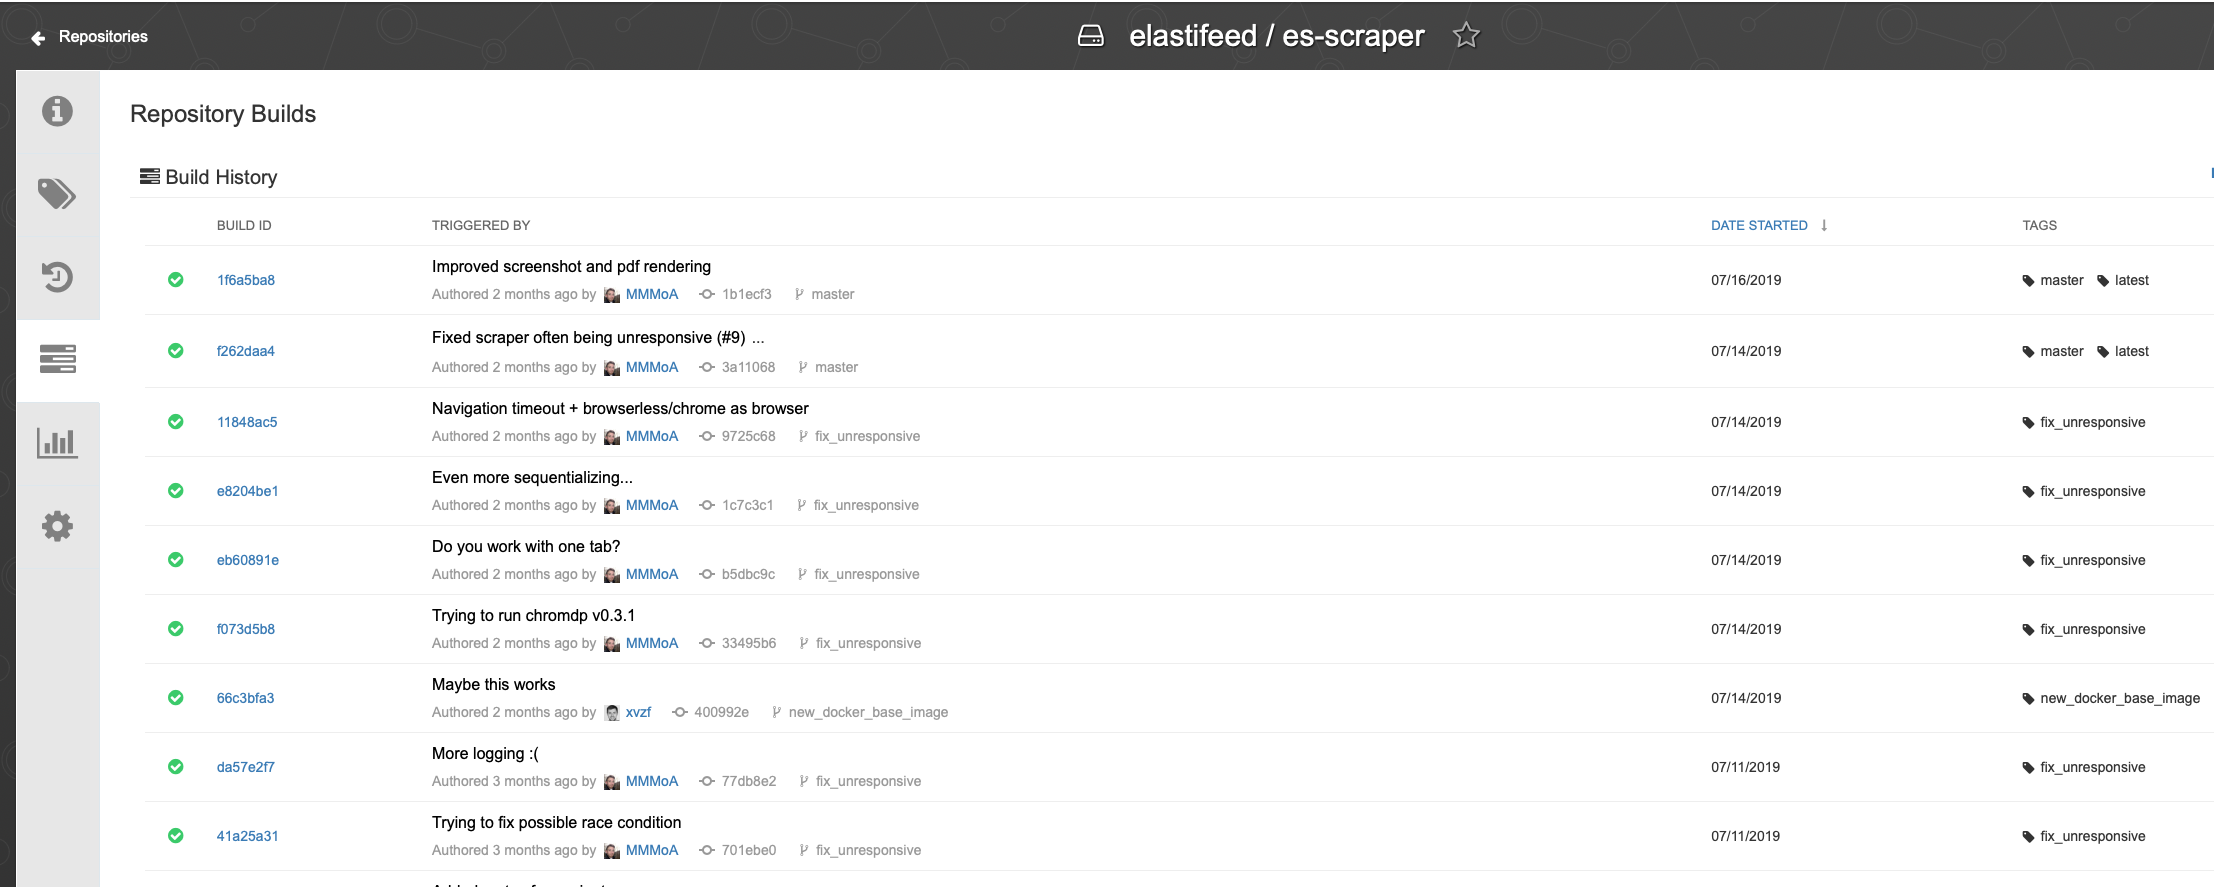
\includegraphics[width=\linewidth]{images/quay.png}
  \caption{Continuous Delivery Pipeline in Quay}
  \label{deployment:image:quay}
\end{figure}

